Para la evaluación y comparación de los modelos entrenados con los
distintos hiperparámetros se recurrió a las mismas métricas que las
referidas en la sección \ref{subsection-results-features}, al evaluar
los posibles vectorizadores.
\par
En este caso, se encontró que los hiperparámetros $C=0.1$ y $penalty=l2$
arrojaron los mejores valores promedios considerando las cinco iteraciones
de la validación cruzada. La única excepción a esto es el resultado en la
métrica de precisión, en el que el modelo entrenado con $C=2$ y $penalty=l2$
obtiene un mejor resultado. No obstante, este modelo muestra los valores
más bajos de cobertura y \textit{F1}. Es notable que, si bien tiene el mayor
valor de precisión observado, esto no llega a compensar su bajo rendimiento
en la cobertura y de ahí que también exhiba el valor de \textit{F1} más bajo.
Con valores más moderados, los demás modelos logran un mejor balance entre
\textit{precision} y \textit{recall}.

\begin{table}[h!]
    \centering
    \begin{adjustbox}{max width=\textwidth}
    \begin{tabular}{ *{7}{|c}| }
    \hline
    Parámetros & \textit{Accuracy} & Precisión & Cobertura & \textit{F1} & \textit{F1-macro} & \textit{F1-weighted} \\
    \hline\hline
    $C=0.1, penalty=l2$ & \cellcolor{highlight-blue!60}0.698 & 0.709 & \cellcolor{highlight-blue!60}0.786  & \cellcolor{highlight-blue!60}0.743 & \cellcolor{highlight-blue!60}0.686 & \cellcolor{highlight-blue!60}0.692 \\
    \hline
    $C=0.5, penalty=l2$ & 0.648 & 0.715 & 0.628  & 0.665 & 0.644 & 0.647 \\
    \hline
    $C=1, penalty=l2$ & \cellcolor{highlight-orange!60}0.622 & \cellcolor{highlight-orange!60}0.695 & 0.583 & 0.6310 & \cellcolor{highlight-orange!60}0.620 & \cellcolor{highlight-orange!60}0.622 \\
    \hline
    $C=2, penalty=l2$ & 0.629 & \cellcolor{highlight-blue!60}0.717 & \cellcolor{highlight-orange!60}0.560 & \cellcolor{highlight-orange!60}0.624 & 0.626 & 0.626 \\
    \hline
\end{tabular}
\end{adjustbox}
\caption{Resultados obtenidos tras evaluar un modelo de Regresión Logística con
distintos hiperparámetos. Los valores reflejan el rendimiento promedio de las
cinco iteraciones de la validación cruzada. Las celdas resaltadas en azul
corresponden a conjunto de hiperparámetros que obtuvo un mejor rendimiento
promedio en cada móetrica de evaluación y las resaltadas en naranja, al
que obtuvo el peor rendimiento.}
\end{table}

Adicionalmente, se graficó la media, el desvío estándar y el valor
obtenido en cada \textit{split} de la métrica \textit{F1}
para cada conjunto de hiperparámetros. Aquí podemos observar que el conjunto
de mejores hiperparámetros no solo presenta un desvío menor que los otros
conjuntos sino que, además, su rendimiento es mejor al resto en todas las
iteraciones.

\begin{figure}[h!]
    \centering
    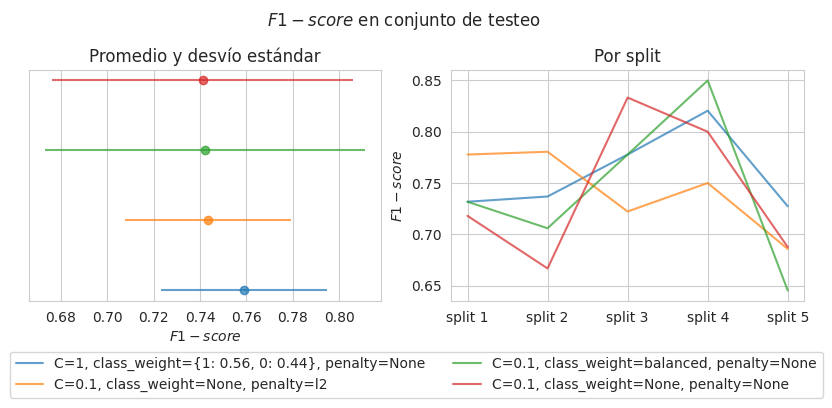
\includegraphics[scale=0.5]{../visualizations/parameters_selection/f1_by_split.png}
    \caption{Contraste}
    \label{fig}
\end{figure}

\begin{table}[h!]
    \centering
    \begin{adjustbox}{max width=\textwidth}
    \begin{tabular}{ *{5}{|c}| }
    \hline
    Clase & Precisión & Cobertura & \textit{F1} & \textit{Soporte} \\
    \hline\hline
    0 (en contra) & 0.80 & 0.67 & 0.73 & 18 \\
    \hline
    1 (a favor) & 0.76 & 0.86 & 0.81  & 22 \\
    \hline\hline
    \textit{Accuray} & & & 0.78 & 40 \\
    \hline
    \textit{Macro AVG} & 0.78 & 0.77 & 0.77 & 40 \\
    \hline
    \textit{Weighted AVG} & 0.78 & 0.78 & 0.77 & 40 \\
    \hline
\end{tabular}
\end{adjustbox}
\caption{Resultado.}
\end{table}


\begin{figure}[h!]
    \centering
    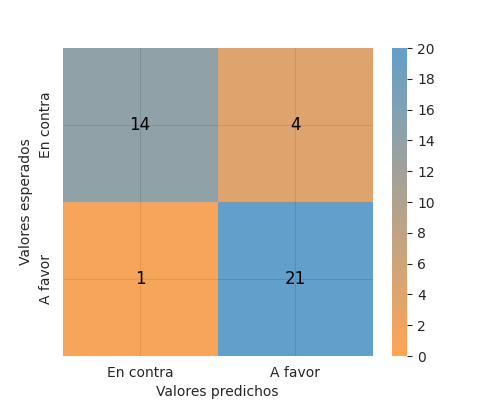
\includegraphics[scale=0.5]{../visualizations/models/confussion_matrix.png}
    \caption{Contraste}
    \label{fig}
\end{figure}

\begin{figure}[h!]
    \centering
    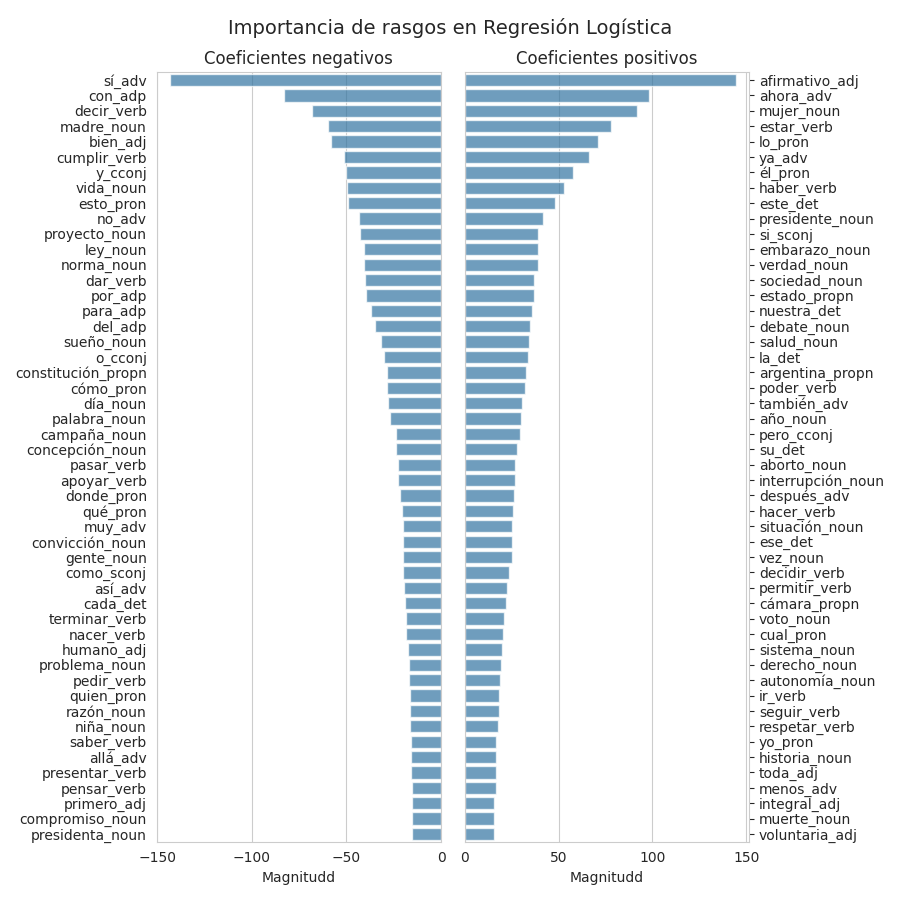
\includegraphics[scale=0.5]{../visualizations/models/lr_feature_importance_barplot_log_proba.png}
    \caption{Contraste}
    \label{fig}
\end{figure}